\documentclass{ctexart}
\usepackage{fancyhdr}
\usepackage{graphicx}
\pagestyle{fancy}
\fancyhf{}

\lfoot{}%这条语句可以让页码出现在下方

\begin{document}
	\title{基于AIoT的智慧消防系统}
	\section{项目方案概述}
	目前,我国智能化消防安全技术远远没有跟上城市急速发展的脚步,因此,我们使用NB-IoT、无线感知、目标检测等技术,将物联网与人工智能、大数据相结合,构建一个系统的智能消防平台。在感知层部署烟雾、温湿度等传感器和摄像头,传感器通过NB-IoT协议接入核心网,向云平台上传感知数据。摄像头通过Wifi或有线的方式入网,向云平台上传视频数据。云平台通过分析多源数据,实现火灾预警、火源识别,并通过视频出分析紧急出口的人流量,实现人员疏散的智能决策。在救援阶段,我们引入了无线感知技术,能够(待补充)。
	\section{项目团队}
	\section{项目产品化}
	\subsection{项目产品特性}
	\subsubsection{基于NB-IoT的温湿度、烟雾监控系统}
	NB-IoT,全称为Narrow Band Internet of Things,中文名窄带物联网,是一个为万物互联打造的新的低功率广域网络。顾名思义,NB-IoT所占用的带宽很窄,只需约180KHz,而且其使用License频段,可采取带内、保护带或独立载波三种部署方式,与现有网络共存,并且能够直接部署在GSM、UMTS或LTE网络,即2/3/4G的网络上,实现现有网络的复用,降低部署成本,实现平滑升级。NB-IoT主要具备以下四大特点:1.广覆盖:相比现有的GSM、宽带LTE等网络覆盖增强了20dB,信号的传输覆盖范围更大(GSM基站目前理想状况下能覆盖35km),能覆盖到深层地下GSM网络无法覆盖到的地方。2.大连接:相比现有无线技术,同一基站下增多了50-100倍的接入数,每小区可以达到50K连接,真是实现万物互联所必须的海量连接。3.低功耗:终端在大部分时间内均处于休眠状态,并集成多种节电技术,待机时间最长可达10年。4.低成本:单NB-IoT通信模块成本不足5美元。因此,我们选择NB-IoT作为通信方式。\par
	该系统的感知层负责采集温度、湿度和烟雾浓度等数据,通过NB-IoT协议接入核心网,通过CoAP协议接入云平台,将采集到的数据上报给云平台。同时,NB-IoT端设备还可以接受云平台下发的指令,并执行响应操作,如触发蜂鸣器警报。
	%我们主要使用了DHT11和MQ-2传感器,DHT11负责采集温湿度、MQ-2负责采集烟雾浓度。如图1所示,我们使用的是EVB\_M1型号的开发板,开发板上搭载stm32微控制单元和BC35通信模块,通过一个类似于手机卡的物联网卡接入核心网,并与云平台通信。物联网端设备的功能是采集现场的温度、湿度和烟雾浓度等数据,并上报给云服务器。云服务器接收到数据后,保存数据、实现数据可视化并分析数据。
	随着物联网的发展,数据量越来越多,各种数据驱动的算法不断应用到物联网系统中来,为用户提供更加便捷的服务,其中,预测性服务是重要的一项。在该系统中,物联网端设备在采集到数据后,仅进行简单的阈值判断,若感知到的数据超过阈值则发出警报。云平台具有更大的存储空间和更强的计算能力,可以基于各个节点采集的历史数据,使用机器学习算法,训练出一个火灾预警模型,该模型能够基于... \par
	\subsubsection{基于深度学习的火焰识别和人流量监测系统}
	随着深度学习的迅猛发展,计算机视觉也成为了目前人工智能领域落地最顺利的技术。计算机视觉(omputer  Vision)是一门研究如何用摄影机和计算机代替人眼对目标进行跟踪、识别、分析、处理等。经过多年的努力,使用计算机视觉软件和硬件算法部署深度学习技术的企业在识别对象方面都取得了一定程度的成功。
	本系统将传感器和视频监控两种方式相结合,主要目的是让二者互补:基于视频监控的方式更直观、更清晰、能够识别出着火的地点,然而摄像头具有视野盲区,且在一些隐私度较高的地点无法部署;基于传感器的监控方式覆盖范围广、数据种类多样化,但不能直观地识别着火区域。两种方式相互结合,既能实现大范围的监控,又能通过视频分析技术识别着火点。
	该系统使用深度学习技术实现了两个目标检测功能,第一个功能是基于YOLOv3算法实现的着火点检测,能够为消防部门的灭火救援提供可靠的信息。第二个是紧急出口的人流量检测,基于人流量信息,能够对人员的疏散进行有序的规划。
	\subsubsection{基于无源感知的人体探测技术}
	\subsection{产品化实施计划}
	该部分主要描述了整个系统的详细架构以及实施部署的方案。
	\subsubsection{基于NB-IoT的温湿度、烟雾监控系统的实现}
	我们基于EVB-M1开发板和华为OceanConnect云平台实现了温湿度、烟雾监控系统。如图1所示,EVB-M1上搭载了BC35-G通信模块(实现了NB-IoT协议的的硬件模块)和stm32微控制单元。传感器我们使用的是DHT11温湿度传感器和MQ2烟雾传感器,DHT11负责采集温度和湿度、MQ2负责采集烟雾浓度。stm32微控制器每隔固定的时间从传感器获取温湿度和烟雾浓度信息,通过BC35-G模块上报给云平台。\par
	\begin{figure}
		\centering
		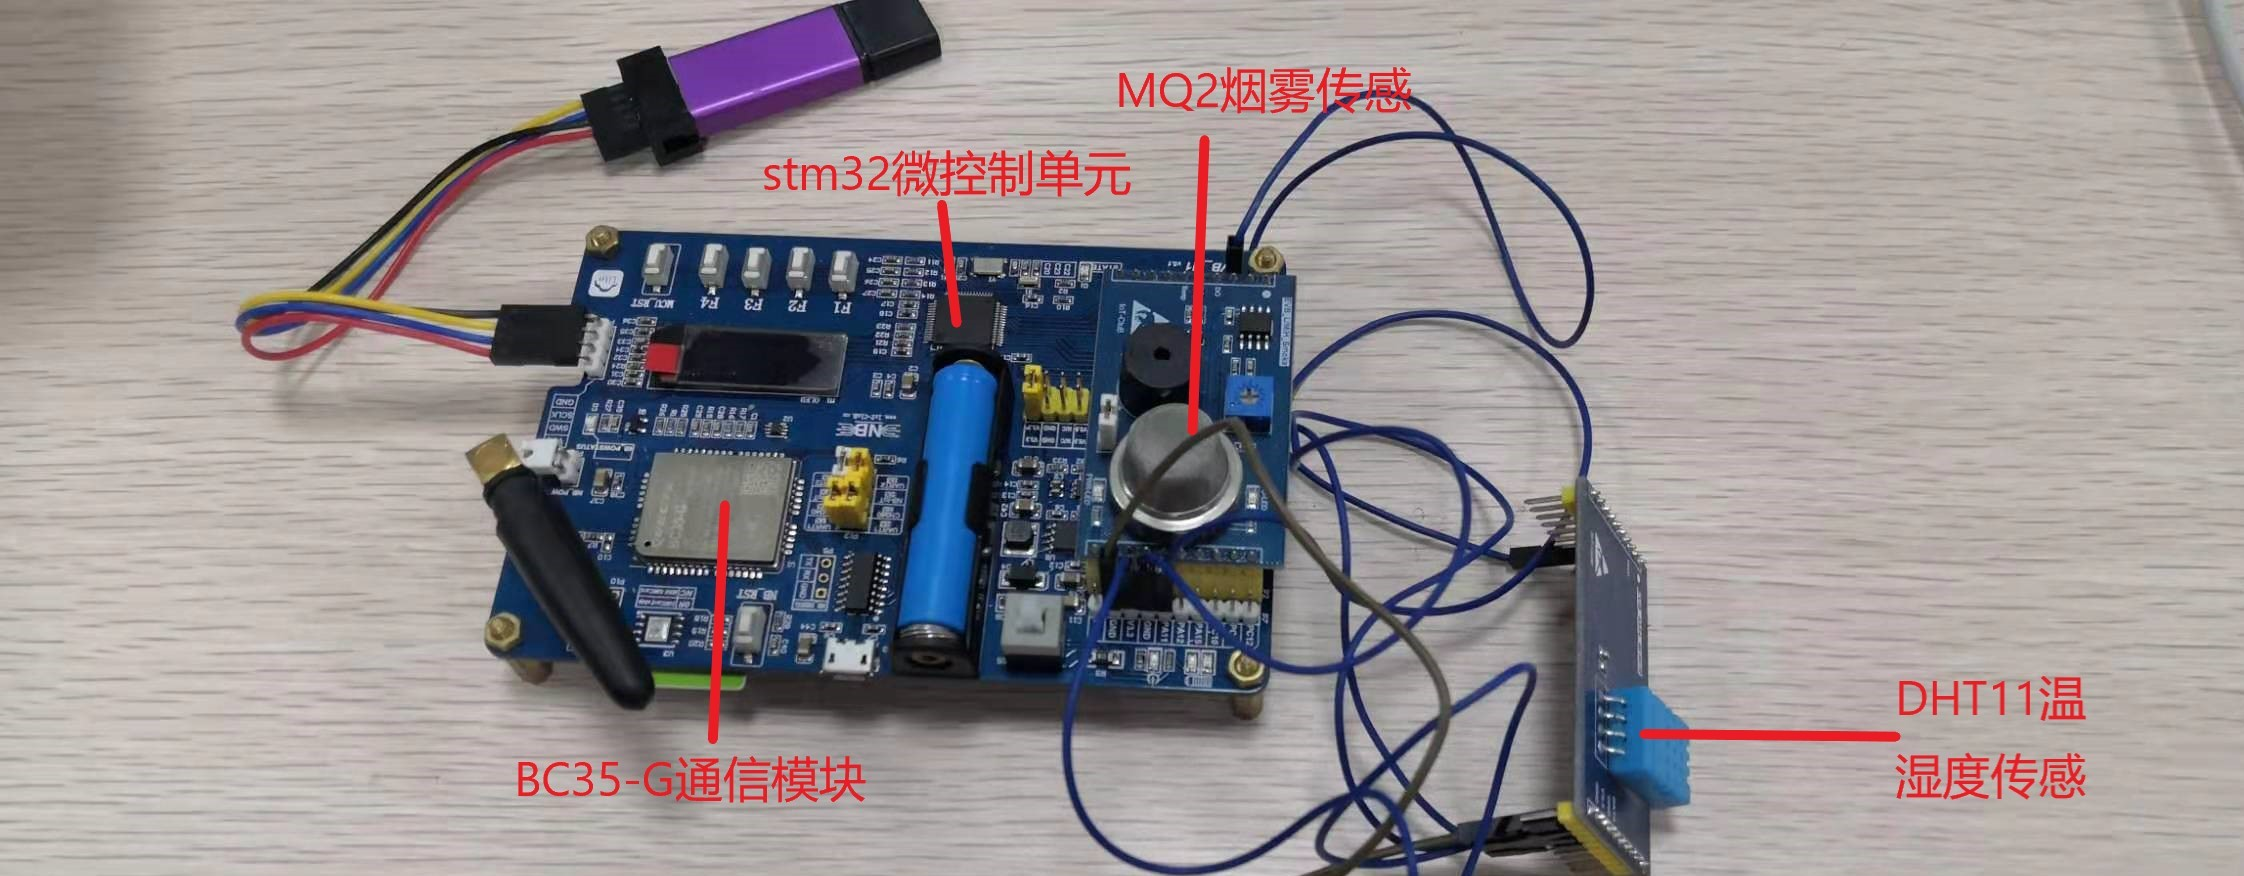
\includegraphics[scale=0.2]{1.jpg}
		\caption{连接传感器的EVB-M1开发板}
		\label{图1}
	\end{figure}
	OceanConnect云平台是华为开发的IoT联接管理平台,通过该平台我们能够很轻易地实现设备的对接、管理和控制。该平台还提供了可视化的Web应用开发功能,我们基于该功能实现了传感器采集数据的实时可视化以及历史数据查看等功能,如图二所示。
	\begin{figure}
		\centering
		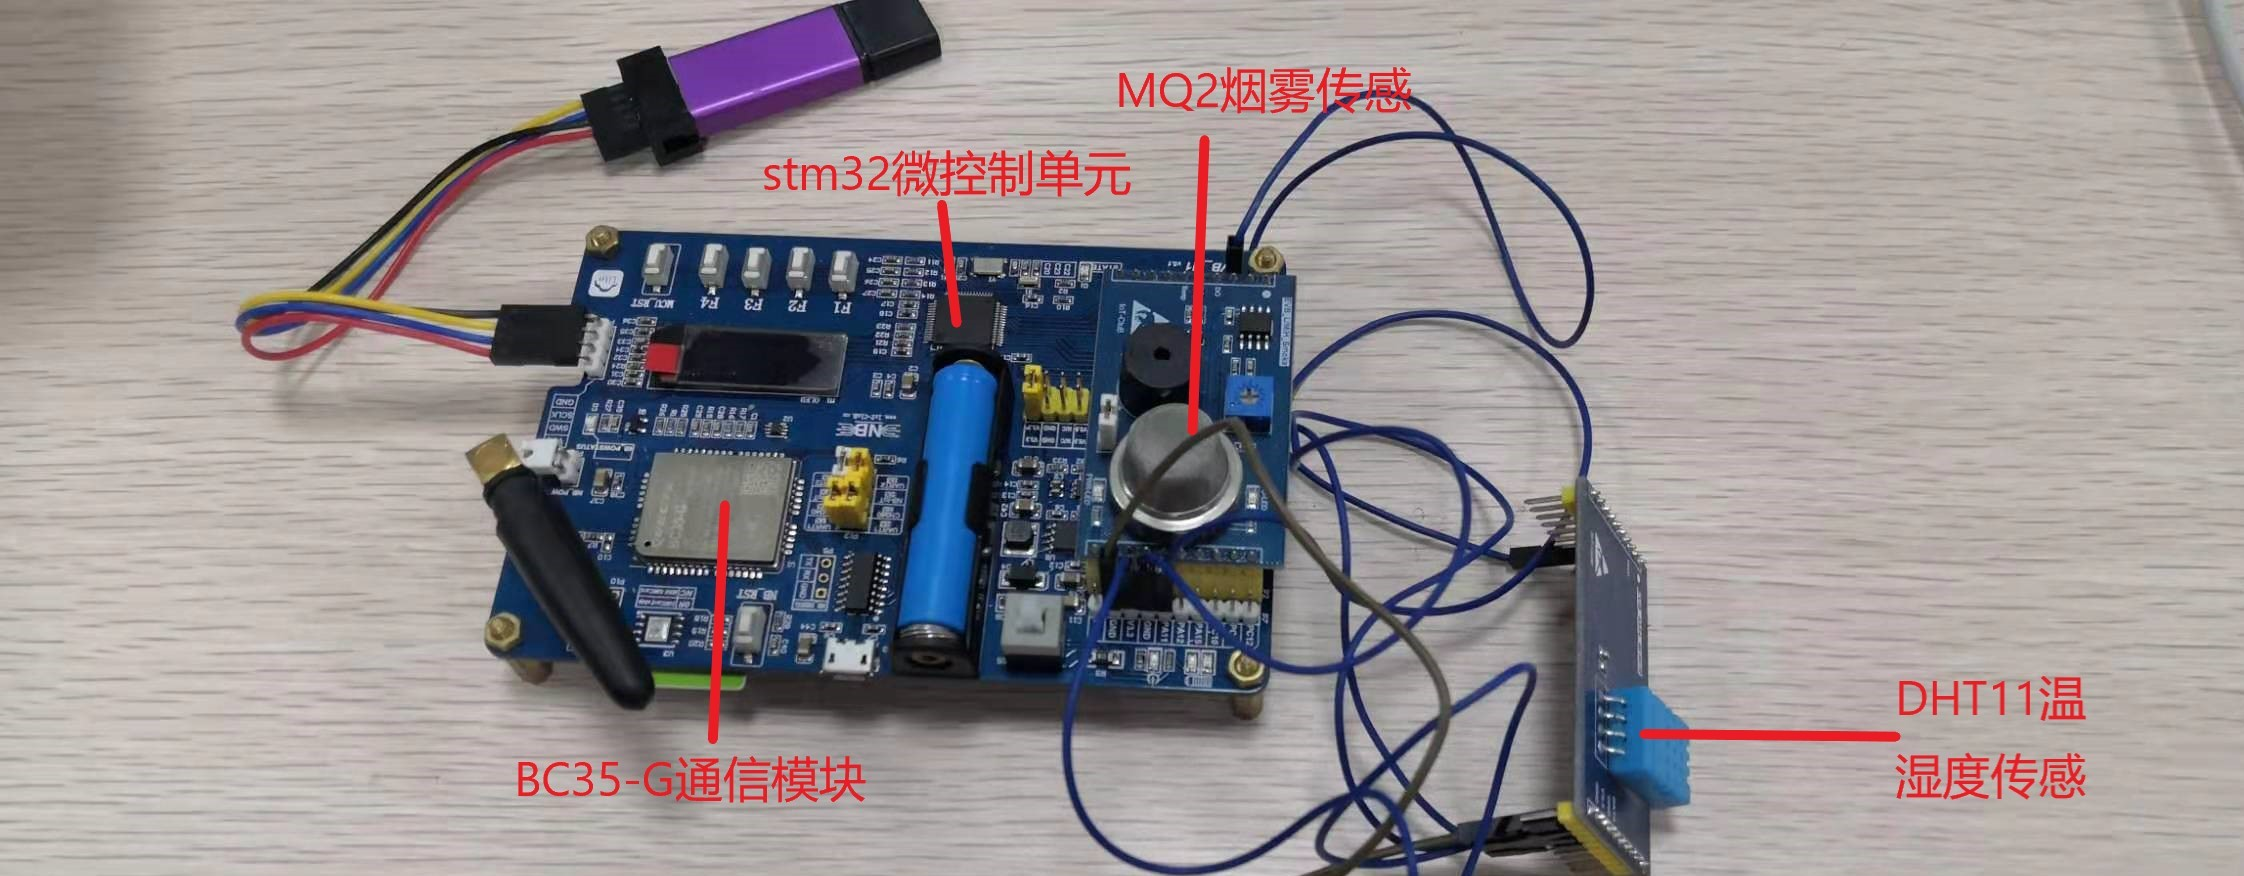
\includegraphics[scale=0.2]{1.jpg}
		\caption{Web应用}
		\label{图2}
	\end{figure}
	\subsubsection{基于深度学习的火焰识别和人流量监测系统的实现}
	我们基于华为ModelArts深度学习平台和opencv等工具实现了基于深度学习的火焰识别和人流量监测。训练一个计算机视觉模型尤其是目标检测模型需要耗费大量的时间和计算资源,因此,我们使用了ModelArts平台部署我们训练好的深度学习模型,ModelArts是面向开发者的一站式AI开发平台,为机器学习与深度学习提供海量数据预处理及半自动化标注、大规模分布式Training、自动化模型生成,及端-边-云模型按需部署能力,帮助用户快速创建和部署模型,管理全周期AI工作流。我们使用YOLOv3算法作为目标检测模型,并在网上收集了300多张室内、室外的火灾图片进行标注,当做训练集,训练了一个火焰检测模型。边缘摄像头将视频数据上传至云服务器,然后云服务器调用ModelArts提供的结构进行视频中的火焰识别,识别效果如图三所示。\par
	\begin{figure}
		\centering
		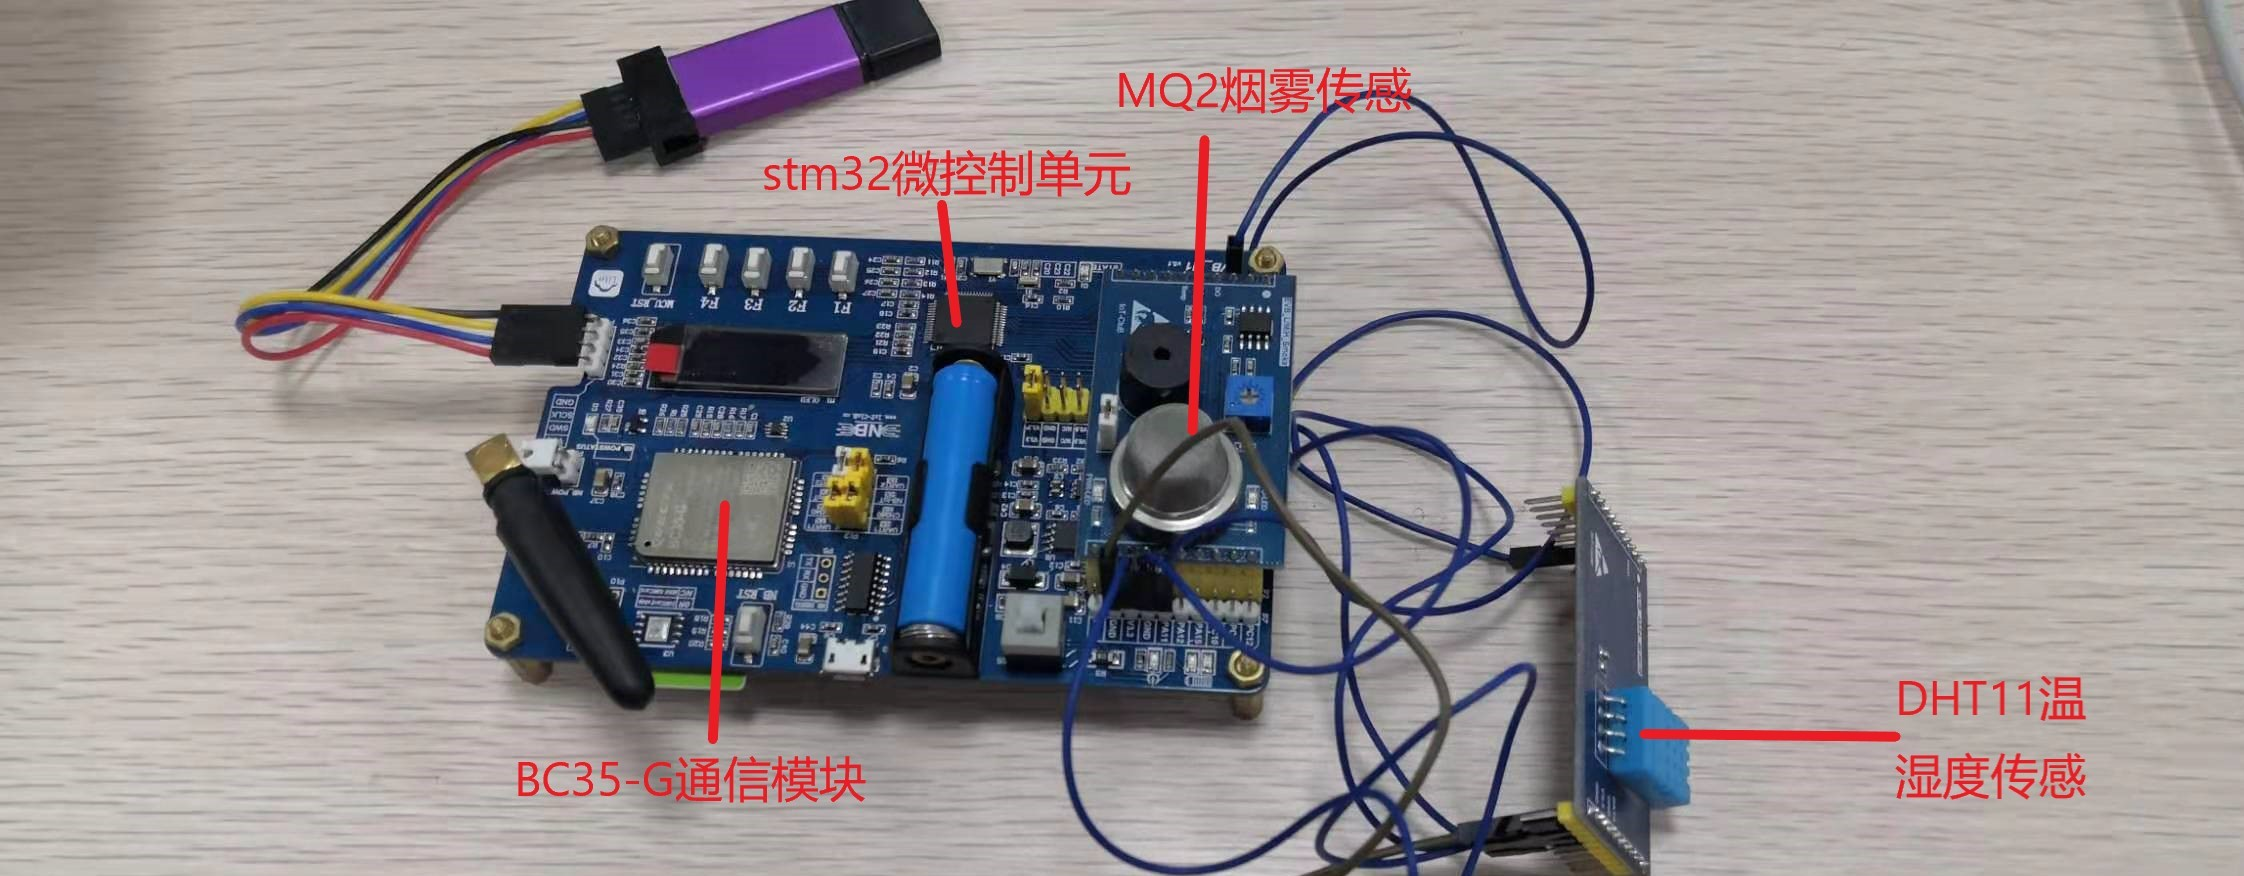
\includegraphics[scale=0.2]{1.jpg}
		\caption{Web应用}
		\label{图2}
	\end{figure}
	同时我们还基于opencv库实现了人流量监测功能。整个系统的架构图如下所示。
	
	
\end{document}